%    Latex Template for ACA 2015
%%%%%%%%%%%%%%%%%%%%%%%%%%%%%%%%%%%%%%%%
%    DO NOT CHANGE THE SETTINGS BELOW
%%%%%%%%%%%%%%%%%%%%%%%%%%%%%%%%%%%%%%%%
\documentclass[11pt]{article}
\usepackage{epsfig}
\usepackage{graphicx}
\usepackage[latin1]{inputenc}
\usepackage[T1]{fontenc}
\usepackage{mathptmx}
\usepackage{url}


%%%%%%%%%%%%%%%%%%%%%%%%%%%%%%%%%%%%%%%%%%%%%%%%%%%%%%%%%%%%%
%%%%%%%%%%% Begin of Autors preabmule settings %%%%%%%%%%%%%%

\usepackage{amsmath, amsfonts, amsthm}
\usepackage{epigraph}
\usepackage{float}

\usepackage{listings,xcolor}

\usepackage{framed}
\colorlet{shadecolor}{gray!20}


\lstset{language=Mathematica}
\lstset{basicstyle={\sffamily\footnotesize},
numberstyle=\tiny\color{gray},
breaklines=true,
captionpos={t},
columns=flexible,
}



\theoremstyle{definition}
\newtheorem{defin}{Definition}

\theoremstyle{definition}
\newtheorem*{example}{Example}


\newcommand{\ds}{\displaystyle}
\newcommand{\R}{\mathbb{R}}
\newcommand{\dx}{\,\mathrm{d}}
\newcommand{\funder}[1]{\underline{#1}\vphantom{#1}}

\newcommand{\sund}{\underline{s\!}\protect\vphantom{s}}

%%%%%%%%%%% End of Autors preabmule settings %%%%%%%%%%%%%%
%%%%%%%%%%%%%%%%%%%%%%%%%%%%%%%%%%%%%%%%%%%%%%%%%%%%%%%%%%%




\begin{document}


%%%%%%%%%%%%%%%%%%%%%%%%
%%%%%%%%%%%%%%%%%%%%%%%%%%%%%%%%%%%%%%%%
%    DO NOT CHANGE THE SETTINGS ABOVE
%%%%%%%%%%%%%%%%%%%%%%%%%%%%%%%%%%%%%%%%
%





\vspace{-0.8cm}
\begin{flushleft}
\Large \textbf{\noindent
%%% PLEASE INSERT THE TITLE OF YOUR TALK HERE %%%%%%%
Familiarizing students with definition of Lebesgue integral  - examples of calculation directly from its definition using Mathematica}
%%%%%%%%%%%%%%%%%%%%%%%%%%%%%%%%%%%%%%%%%%%%%%%%%%%%%%%%
\\
%%%%%%%%%%%%%%%%%%%%%%%%%%%%%%
\vspace{0.5cm}
\normalsize
 %%%%%%             NAMES OF AUTHORS         %%%%%%
 %%%%%% NAME OF SPEAKER SHOULD BE UNDERLINED %%%%%%%%%
\normalsize{
 %%%%%% FOR EXAMPLE %%%%%
\underline{ W{\l}odzimierz Wojas$^1$}, \underline{Jan Krupa}$^2$
 %%%%%%%%%%%%%%%%%%%%%%%%
} \\
\vspace{5mm}
\textit{\footnotesize
 %%%%%% AFFILIATION OF AUTHORS %%%%%%
$^1$ Warsaw University of Life Sciences (SGGW), Poland, {\tt wlodzimierz\_wojas@sggw.pl}\\
$^2$ Warsaw University of Life Sciences (SGGW), Poland, {\tt jan\_krupa@sggw.pl}\\
 %%%%%%%%%%%%%%%%%%%%%%%%%%%%%%%%%%%%%
}
\end{flushleft}

\epigraph{\textit{``Young man, in mathematics you don't understand things. You just get used to them''}}{John von Neumann}


In popular books of calculus, for example \cite{Apostol, Ficht}, we can find many examples of Riemann integral calculated directly from its definition. The aim of these examples is to familiarize students with the definition of Riemann integral. But we cannot find analogical examples for Lebesgue integral. In this article, with similar aim but for Lebesgue integral definition,  we present the following examples of calculation directly from its definition: $\ds \int_0^1 x^2 \dx m(x)$, $\ds \int_0^1 x^k \dx m(x)$, $\ds \int_0^{\pi/2} \sin x \dx m(x)$, $\ds \int_a^b \exp(x) \dx m(x)$, $\ds \int_0^{\pi}\ln(1-2r \cos x+r^2) \dx m(x)$, where $\ds \dx m(x)$ denotes the Lebesgue measure on the real line. We calculate sums, limits and plot graphs of needed simple functions using Mathematica.  The two following definitions of Lebesgue integral are used in this article:

Let $(\R, \mathfrak{M}, m)$ be measure space, where
$\mathfrak{M}$ is $\sigma-$ algebra of Lebesgue measurable subsets
in $\R$, and $m$- Lebesgue measure on  $\R$.

Let $f:\R \to \R$ be measurable nonnegative function (we've  omitted the definition of Lebesgue integral for simple real measurable functions).

\begin{defin} (See \cite{Rudin, Bartle, Jones, Browder, Folland})
\label{def:1}
\begin{equation}
\label{eq:1}
\int f\dx m(x) = \sup \Big\{ \int s\dx m(x): 0\leq s \leq f, s\; \mathrm{simple\;measurable\; function}\Big\}.
\end{equation}
\end{defin}

\begin{defin} (See \cite{Char, Kol, Sik})
\label{def:2}
Let $s_n$ be nondecreasing sequence of nonnegative simple measurable functions such that $\ds \lim_{n\to \infty}s_n (x)=f(x)$ for every $x\in \R$.
Then:
%converging to $f$ as $n$ approaches to infinity.
\begin{equation}
\label{eq:2}
\int f\dx m(x) = \lim_{n\to \infty}\int s_n \dx m(x).
\end{equation}
\end{defin}



\begin{example}
Let consider the function: $\ds f(x) = \sin x, x\in [0,\pi/2)$. For the rest of this example we will restrict our consideration to $x \in [0, \pi/2)$.\\
We will calculate $\ds \int_0^{\pi/2} \sin x \dx m(x)$ applying directly definition \ref{def:1}.

\noindent
Consider

\noindent
$\ds \underline{s\!}\vphantom{s}_n(x) =
\sum_{k=0}^{2^n-1}
\sin \bigg(\frac {k}{2^{n+1}} \pi \bigg)\chi_{\big[\frac {k}{2^{n+1}} \pi, \frac{k+1}{2^{n+1}} \pi\big)}(x)$,
for $x\in [0,\pi/2)$, $ n=1,2,\ldots$\\
and
$\ds \bar{s}_n(x) = \bar{s}_n=
\sum_{k=1}^{2^n}
\sin \bigg(\frac {k}{2^{n+1}} \pi\bigg)\chi_{\big[\frac {k-1}{2^{n+1}} \pi, \frac{k}{2^{n+1}} \pi\big)}(x)$,
for $x\in [0,\pi/2)$,  $ n=1,2,\ldots$.

\noindent
Using Wolfram Mathematica we get the following Figures \ref{fig:1}, \ref{fig:2}:
\begin{figure}[H]
\begin{center}
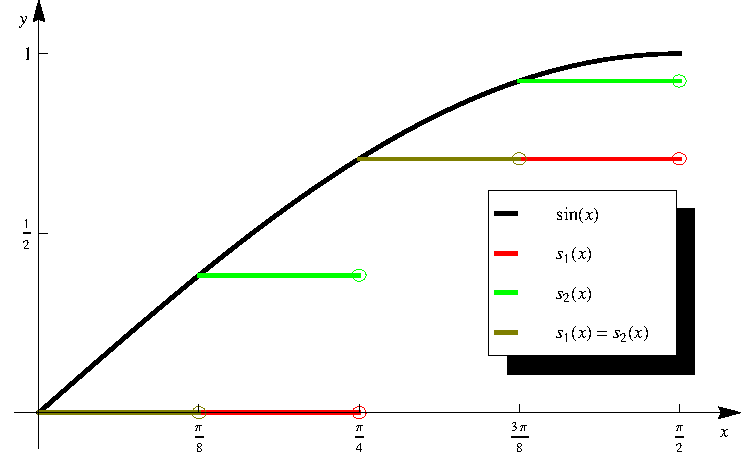
\includegraphics[scale=0.7]{fig1L.pdf}
\caption{Graphs of functions $f$, $\ds \sund_1, \sund_2$. We can see that $\ds \sund_1(x)\leq \sund_2(x)$ for $x\in [0, \pi/2)$.}
\label{fig:1}
\end{center}

\end{figure}


\begin{figure}[H]
\begin{center}
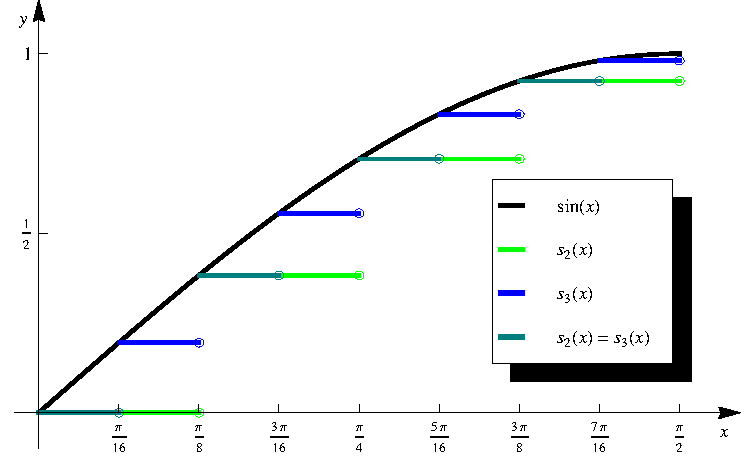
\includegraphics[scale=0.7]{fig2L.pdf}
\caption{Graphs of functions $f$, $\ds \sund_2, \sund_3$. We can see that $\ds \sund_2(x)\leq \sund_3(x)$ for $x\in [0, \pi/2)$.}
\label{fig:2}
\end{center}
\end{figure}


\noindent
It is clear that  $\ds \funder{s}_n$, $\ds \bar{s}_n$ are  sequences of nonnegative simple measurable functions and that  $\ds \funder{s}_n \leq f$
and $\ds \bar{s}_n \geq f$ on $\ds [0, \pi/2)$ for  all $n=1,2, \ldots$.\\

\noindent
Using Wolfram Mathematica we get:
{\normalfont
\begin{shaded*}
\setlength{\fboxsep}{0pt}
\begin{lstlisting}[language=Mathematica,caption=Mathematica code:\label{lst:1}]
In[1]=Sum[Sin[Pi k/2^(n+1)], {k, 0, 2^n-1}] Pi/2^(n+1)//Simplify
Out[1]=2^(-2-n)Pi(-1+Cot[2^(-2-n)Pi])

In[2]=Limit[%,n->Infinity]
Out[2]=1
\end{lstlisting}
\end{shaded*}
}
\noindent
So
\begin{equation}
 \label{eq:3}
 \funder{a}_n=\int \funder{s}_n \dx m)x) = \sum_{k=0}^{2^n-1}\sin\frac{k\pi}{2^{n+1}}\cdot \frac {1}{2^{n+1}}\pi = 2^{-2-n}\pi(-1+\cot(2^{-2-n}\pi))\to 1
 \end{equation}
Similarly
{\normalfont
\begin{shaded*}
\begin{lstlisting}[language=Mathematica,caption=Mathematica code:\label{lst:2}]
In[3]=Sum[Sin[Pi k/2^(n+1)], {k, 1, 2^n}] Pi/2^(n+1)//Simplify
Out[3]=2^(-2-n)Pi(1+Cot[2^(-2-n)Pi])

In[4]=Limit[%,n->Infinity]
Out[4]=1
\end{lstlisting}
\end{shaded*}
}
\noindent
So
\begin{equation}
 \label{eq:4}
 \bar{a}_n=\int \bar{s}_n \dx m(x) =
\sum_{k=1}^{2^n}\sin\frac{k\pi}{2^{n+1}}\cdot \frac {1}{2^{n+1}}\pi = 2^{-2-n}\pi(1+\cot(2^{-2-n}\pi))\to 1\\
\end{equation}

\noindent
Of course we could use the following formulae: $\ds \sum_{k=1}^n\sin(kx)=\frac{\sin\frac{n+1}{2}x\sin\frac{n}{2}x}{\sin\frac{x}{2}}$ and $\ds \lim_{x\to 0}\frac{\sin x}{x}=1$ instead of the code in Listings \ref{lst:1} and \ref{lst:2}
to get the results in formulae (\ref{eq:3}) and (\ref{eq:4}).

\quad

\noindent
Using formulae (\ref{eq:3}) and (\ref{eq:4}),  basic properties of least upper, greatest lower bounds and of Lebesgue integral of simple measurable functions we will prove in our talk that:
\begin{equation}
\label{eq:5}
\ds \sup \Big\{ \int s\dx m(x): 0\leq s \leq f, s\; \mathrm{simple\;measurable\; function}\Big\}
\geq 1
\end{equation}
and
\begin{equation}
\label{eq:6}
\ds \sup \Big\{ \int s\dx m(x): 0\leq s \leq f, s\; \mathrm{simple\;measurable\; function}\Big\}
\leq 1.
\end{equation}
Inequalities (\ref{eq:5}) and (\ref{eq:6}) give
$$
\sup \Big\{ \int s\dx m(x): 0\leq s \leq f, s\; \mathrm{simple\;measurable\; function}\Big\} =
1,
$$
which means that
$\ds \int f\dx m(x) = \int \sin x\dx m(x) =1.$


\noindent
Let calculate $\ds \int \sin x \dx m(x)$ applying directly definition \ref{def:2}.

\noindent
We can see that $\ds \funder{s}_n(x)\leq \funder{s}_{n+1}(x)$ for $x\in [0, \pi/2)$ and for all $n=1,2,\ldots$.
In Figures \ref{fig:1} and \ref{fig:2} we can see that $\ds \funder{s}_1(x)\leq \funder{s}_2(x)$ and $\ds \funder{s}_2(x)\leq \funder{s}_3(x)$ for $x\in [0, \pi/2)$.
W can also see that $\ds \lim_{n\to \infty} \funder{s}_n(x)=\sin(x)$ for all $x\in [0, \pi/2)$. So $\ds \funder{s}_n$ is nondecreasing sequence of nonnegative simple measurable functions and  $\ds \funder{s}_n$ converges pointwise to $f$.

\noindent
So by formula (\ref{eq:3}) and directly by definition \ref{def:2} we get $\ds \int \sin x\dx m(x) = \int f\dx m(x) = \lim_{n\to \infty} \int \funder{s}_n \dx m(x)= \lim_{n \to \infty}  \funder{a}_n =1$.



\end{example}

%%%%%%%%%%%%%%%%%%%%%%%%%%%%%%%%%%%%%%%%
%% BIBLIOGRAPHY
%%%%%%%%%%%%%%%%%%%%%%%%%%%%%%%%%%%%%%%%
\begin{thebibliography}{00}
\addcontentsline{toc}{chapter}{References}

\setlength{\itemsep}{-1mm}
\footnotesize
\bibitem{Apostol} Tom M. Apostol, \textit{Calculus, Volume 1, One-Variable Calculus with an Introduction to Linear Algebra}, 2\textsuperscript{nd} ed., Addison-Wesley Publishing Company, (1991)
\bibitem{Ficht} G. M. Fichtenholz, \textit{Differential and Integral Calculus}, Fizmatgiz, (1958)
\bibitem{Rudin} W. Rudin, \textit{Principles of Mathematical Analysis}, 3\textsuperscript{rd} ed., McGraw-Hill Education, (1973)
\bibitem{Char}  Charalambos D. Aliprantis, Owen Burkinshaw, \textit{Principles of Real Analysis}, 3\textsuperscript{rd} ed., Academic Press,  (1998)
\bibitem{Bartle} Robert G. Bartle, \textit{The Elements of Integration and Lebesgue Measure}, Wiley-Interscience, (1995)
\bibitem{Jones} Frank Jones, \textit{Lebesgue Integration On Euclidean Space}, Jones \& Bartlett Learning, (2000)
\bibitem{Browder} Andrew Browder, \textit{Mathematical Analysis An Introduction}, 2\textsuperscript{nd} ed.,  Springer, (2001)
\bibitem{Folland} Gerald B. Folland,  \textit{Real Analysis Modern Technique}, 2\textsuperscript{nd} ed., Wiley, (2007)
\bibitem{Kol} W. Ko{\l}odziej, \textit{Mathematical Analysis}, (in polish), Polish Scientific Publishers PWN, Warsaw (2012)
\bibitem{Sik} R. Sikorski, \textit{Differential and Integral Calculus. Functions of several variables},  (in polish), Polish Scientific Publishers PWN, Warsaw (1977)
\bibitem{Ruskeepa} H. Ruskeepa \textit{Mathematica Navigator: Graphics and Methods of applied Mathematics.}
Academic Press, Boston (2005)
\bibitem{Wolfram}
S. Wolfram  \textit{The Mathematica Book.} Wolfram Media/ Cambridge University Press (1996)
\end{thebibliography}
\normalsize

\end{document}
